\section{Breadth-First Search (BFS)} \index{breadth-first search (BFS)}

\subsection{BFS Algorithm}
Given a graph $G=(V,E)$ and a distinguished source vertex $s$, breadth-first search systematically explores the edges of $G$ to discover every vertex that is reachable from $s$. Breadth-first search expands the frontier between disvoered and undiscovered vertices uniformly across the breadth of the frontier. The algorithm discovers all vertices at distance $k$ from $s$ before discovering any vertices at distance $k+1$.

BFS visits all the vertices in a connected undirected graph in order of their distance from the start vertex $s$. As we visit the nodes, we can also determine $\delta(s,v)$ which is the distance from $s$ to $v$, that is, the number of edges on the shortest path from $s$ to $v$.

\begin{codebox}
    \Procname{$\proc{BFS}(s)$}
    \li $Q = \proc{Queue}(\{\})$;\; $d = [ \, ]$ 
    \li \For $v \in V$ \Do
        \li $d[v] = 0$ 
        \li label $v$ as unvisited \End
    \li visit $s$
    \li $\color{cyan} \pi[s] = \const{nil}$ 
    \li $\proc{Enqueue}(Q,s)$
    \li \While $Q \neq \emptyset$ \Do
        \li $u = \proc{Head}(Q)$
        \li \For {\color{cyan}out} neighbor $v$ of $u$ \Do
            \li \If $v$ is unvisited \Then
                \li $\proc{Enqueue}(Q,v)$
                \li $d[v] = d[u] + 1$
                \li \color{cyan} $\pi[v] = u$  \End
            \End
        \li $\proc{Dequeue}(Q)$
\end{codebox}

We keep track of the shortest length from $s$ to each vertex in the array $d$. We will prove the correctness of BFS for calculating shortes path in a later subsection.

If $G$ is not connected, this algorithm visits the connected component of $G$ containing $s$. If $G$ is directed, this visits all vertices reachable from $s$ by a directed path.

\subsection{Edge Classification}

We can create a tree, known as BFS tree, by running the BFS algorithm on a graph. Each level of the BFS tree contains vertices reachable with one step from their corresponding parents at the previous level.

Using the BFS tree, we can classify edges in a graph into three categories:

\begin{itemize} \index{tree edge} \index{cross edge} \index{back edge}
    \item Tree edge ({\color{seagreen} green}): $\{v,\, \attrib{v}{parent}\}$ or $(\attrib{v}{parent},\, v)$ if directed.
    \item Cross edge ({\color{orange} orange}): $\{ u,v \}$ or $(u,v)$ if directed where $u$ is not an ancestor of descendant of $v$ in the BFS tree.
    \item Back edge ({\color{red} red}): edge from a node to one of its ancestors.
\end{itemize}

\begin{figure}[htbp]
    \centering
    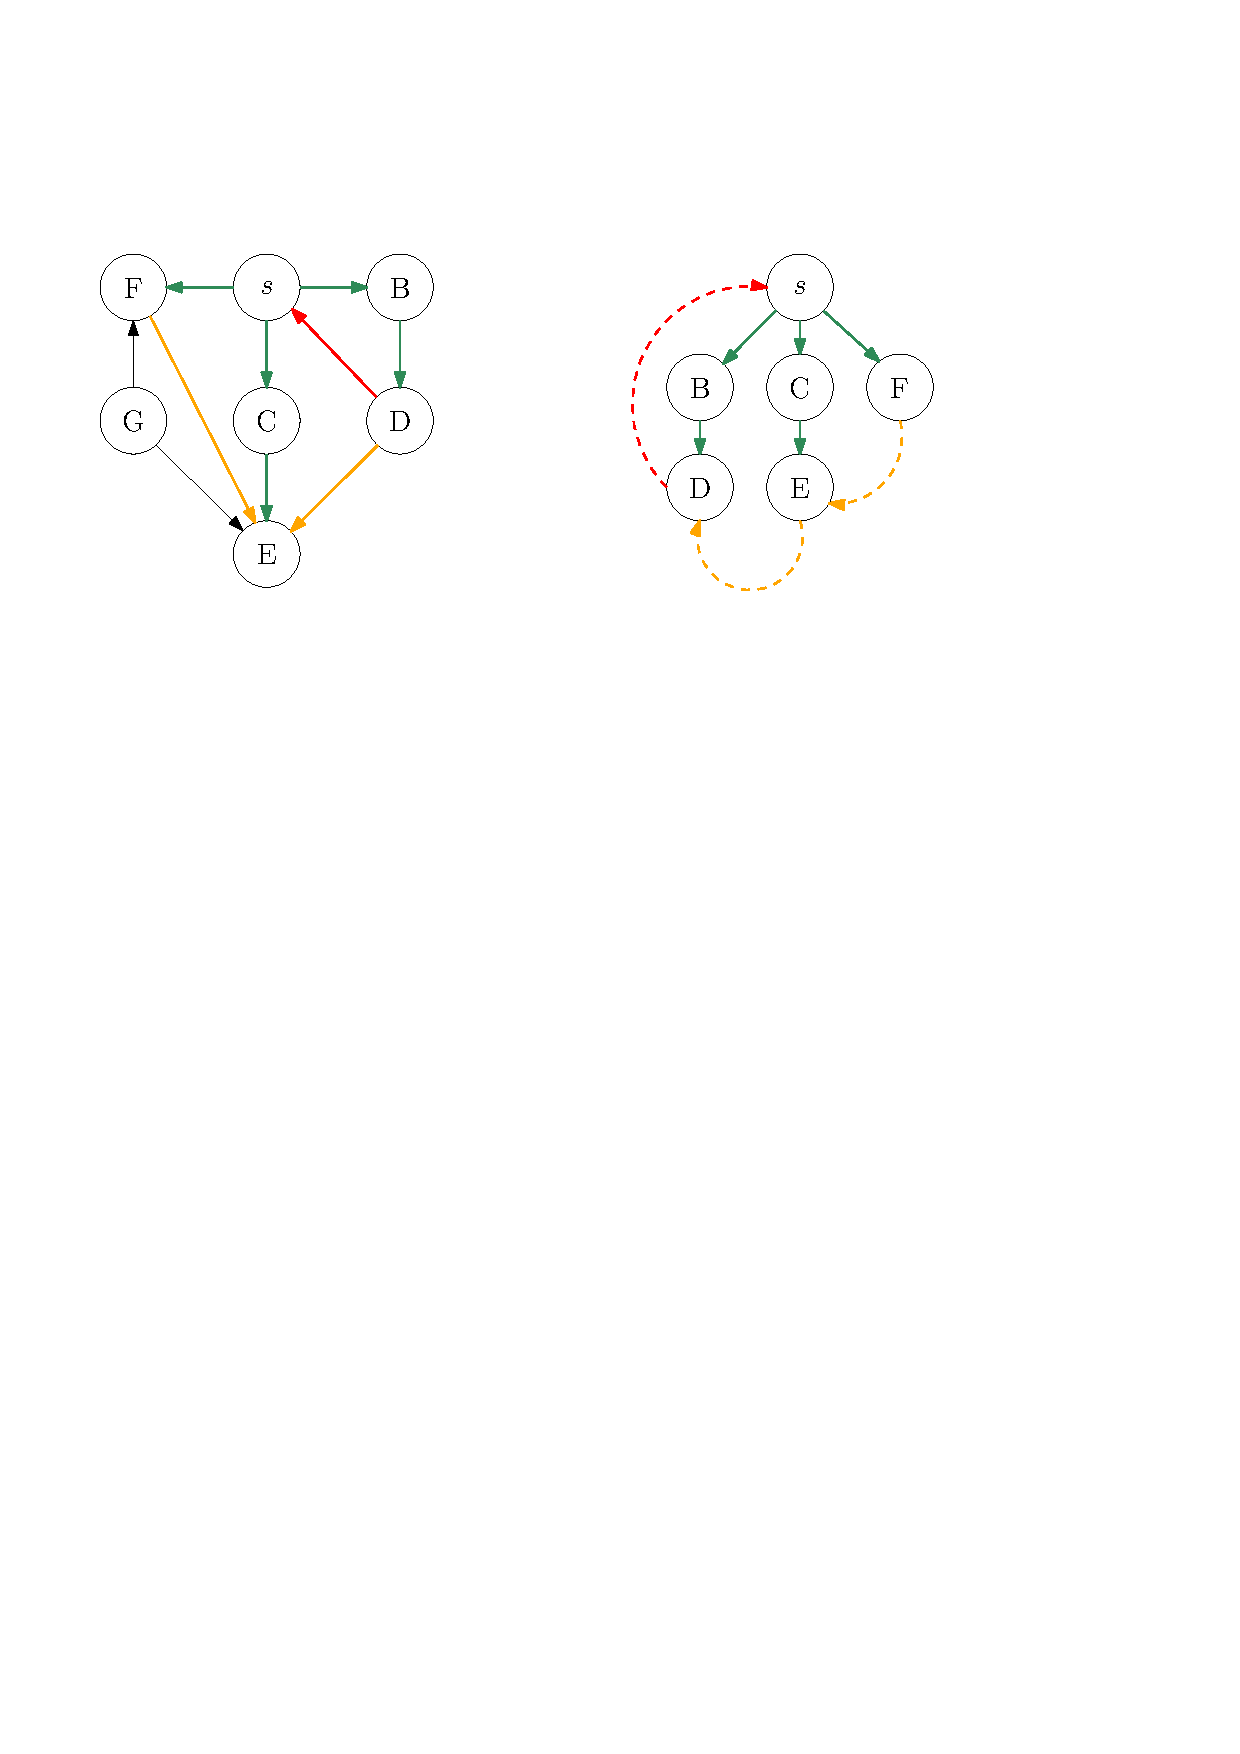
\includegraphics[width=0.7\linewidth]{bfs/bfs-example.pdf}
    \caption{A graph and its corresponding BFS tree. Edges are colored based on their classification.}
    \label{fig:bfs-example}
\end{figure}

\begin{lemma}
    If $G$ is undirected, then all edges are tree edges or cross edges.
\end{lemma}

\begin{proof}
    Suppose that $\{u,v\}$ is a back edge discovered when $u$ is at the head of $Q$.

    Since $v$ is an ancestor of $u$, it was visited and hence enqueued before $u$. So $v$ was the head of $Q$ before $u$. Since $\{u,v\} \in E$, $u$ was visited when $v$ was at the head of $Q$.This means that $\{u,v\}$ is a tree edge.
\end{proof}

\subsection{Correctness of BFS}

\textit{Claim}. If $G$ is connected, then at the end of BFS, $d[v] = \delta(s,v)$ for all $v \in V$.

\textit{Observation}. $d[v]=0$ if and only if $v=s$. If $G$ is directed, $(\pi[v],\, v) \in E$. If $G$ is undirected, $\{ \pi[v], v \} \in E$. $d[v] = d[\pi[v]]+1$.

From this observation, we have the following lemma.

\begin{lemma}
    At the end of the BFS, $d[v] \geq \delta(s,v)$ for all nodes reachable from $s$.
\end{lemma}

\begin{proof}
    $d[v]$ is the length of the path from $s$ to $v$ in the BFS tre since $d[v] = d[\pi[v]] + 1$ for all nodes $v \neq s$ reachable from $s$.

    All these edges are in $E$, so $\delta(s,v) \leq d[v]$.
\end{proof}

\begin{lemma}
    Let $s=v_1,v_2,\cdots,v_n$ be the nodes in the order they are visited (enqueued). Then, $0=d[v_1] \leq \cdots \leq d[v_n]$. 
\end{lemma}

\begin{proof}
    Suppose not. Let $j>1$ be the smallest integer such that $d[v_{j-1}] > d[v_j]$.
    
    Let $v_h = \pi[v_{j-1}]$ where $h < j-1$, and let $v_i = \pi[v_j]$ where $i < j$.
    
    $d[v_{j-1}] = 1 + d[v_{h}]$ and $d[v_j] = 1 + d[v_i]$. Since $d[v_{j-1}] > d[v_j]$, then $d[v_h] > d[v_i]$. Since $h,i \leq j-1$ and $d[v_1] \leq \cdots \leq d[v_{j-1}]$, it follows that $i<h$. So, $d[v_j] \leq d[v_i]$ and $d[v_h] \leq d[v_{j-1}]$.

    This means $v_i$ is enqueued and hence dequeued before $v_h$, which then implies that $v_j$ was enqueued before $v_{j-1}$. This is a contradiction.
\end{proof}

Alternatively, this lemma can also be proved using induction on the number of queue operations (see CLRS pp 599).

Finally, using the lemmas that we have proved, we can show that BFS correctly calculates the shortest path from $s$ to all vertices reachable from $s$.

\begin{theorem}
    At the end of $\proc{BFS}(s)$, $d[v] = \delta(s,v)$ for all nodes $v$ reachable from $s$.
\end{theorem}

\begin{proof}
    Consider the shortest path (of length) $\delta(s,v)$ from $s$ to $v$ in $G$. Let $\{u,v\}$ be the last edge in this path where $u$ is the parent of $v$ on that path. $\delta(s,u) = \delta(s,v) - 1$. $\delta(s,s) = 0 = d[s]$.

    Let $v$ be a vertex where the theorem is not ture. That is, let $v$ be a vertex with minimum value of $\delta(s,v)$ such that $d[v] > \delta(s,v)$. Let $u$ be the predecessor of $v$ on the shortest path from $s$ to $v$. Then, we know that $\delta(s,u) = d[u]$ and $\delta(s,v) = d[v] = d[\pi[v]]+1$. So, $d[v] > d[u] + 1$. 
    
    Consider the two cases: If $v$ was unvisited, then $d[v] = d[u] + 1$ after the execution, which is a contradiction. If $v$ has been visited, there exists a $\pi[v]$ in the BFS tree that was dequeued and thus enqueued before $u$. By Lemma, $d[\pi[v]] \leq d[u]$. Hence $d[v] = d[\pi[v]] + 1 \leq d[u] + 1$, which is a contradiction. No such $v$ exists. Therefore, the theorem holds.
\end{proof}

\subsection{Running Time of BFS}

If represented using an adjacency list, the BFS algorithm is $O(n+m)$. Each node $v$ is enqueued at most once. Its adjacency list is examined at most once. If represnted using an adjacency matrix, it requires $\Theta(n^2)$ time.
